\section{前缀和(扫描):并行算法工作效率介绍}
我们的下一个并行模式是前缀和,通常也称为扫描。 并行扫描经常用于并行化看似顺序的操作,例如资源分配、工作分配和多项式求值。 
一般来说,如果计算自然地被描述为数学递归,其中系列中的每个项都是根据前一个项来定义的,
那么它很可能被并行化为并行扫描操作。 并行扫描在大规模并行计算中发挥着关键作用,
原因很简单:应用程序的任何顺序部分都会极大地限制应用程序的整体性能。 许多这样的连续部分可以通过并行扫描转换为并行计算。 
因此,并行扫描通常用作并行算法中的基本操作,执行基数排序、快速排序、字符串比较、多项式求值、求解递归、树操作和流压缩。 
基数排序示例将在第 13 章“排序”中介绍。

并行扫描是一种重要的并行模式的另一个原因是,它是一些并行算法执行的工作可能比顺序算法执行的工作具有更高复杂性的典型示例,
从而导致需要在 算法复杂度和并行化。 正如我们将要展示的,
算法复杂性的轻微增加可能会使并行扫描比大型数据集的顺序扫描运行得更慢。 
在“大数据”时代,这种考虑变得更加重要,因为海量数据集对计算复杂度较高的传统算法提出了挑战。

\subsection{背景}
从数学上讲,包含(inclusive) 扫描操作需要一个二元关联运算符 $\oplus$ 
和一个由 $n$ 个元素组成的输入数组 $\left[x_{0}, x_{1}, \ldots, x_{n-1}\right] $,并返回以下输出数组:
$$
\left[x_{0}, \quad\left(x_{0} \oplus x_{1}\right), \ldots,\left(x_{0} \oplus x_{1} \oplus \ldots \oplus x_ {n-1}\right)\right]
$$

例如,如果 $\oplus$ 是加法,则对输入数组 $[\begin{array}{llllllll}
3 & 1 & 7 & 0 & 4 & 1 & 6 & 3
\end{array}$ 进行包含扫描操作将返回 
$[2,3+1,3+1+7,3+1+7+0, \ldots, 3+1+7+0+4+1+6+3]$ $ =[\begin{array}{llllllll}
3 & 4 & 11 & 11 & 15 & 16 & 22 & 25
\end{array}]$. “包含(inclusive)”扫描这个名称来源于这样一个事实:每个输出元素都包含相应输入元素的效果。

我们可以使用为一群人切香肠的示例来说明包含扫描操作的应用。 假设我们有一根 40 英寸的香肠可供八个人享用。 
每个人都订购了不同的英寸数量: $3,1,7,0,4,1,6$ 和 3 。 
也就是说,人员 0 想要 3 英寸的香肠,人员 1 想要 1 英寸,依此类推。 我们可以顺序或并行地切香肠。 顺序方式非常简单。 
我们首先为第 0 号人员切下 3 英寸的部分。香肠现在长 37 英寸。 然后我们为第 1 个人切一段 1 英寸的部分。
香肠变成 36 英寸长。 我们可以继续切割更多的部分,直到我们将 3 英寸的部分提供给第 7 个人。 
至此,我们总共已经提供了 25 英寸的香肠,还剩下 15 英寸。

通过包含扫描操作,我们可以根据每个人订购的数量计算出所有切割点的位置。 
也就是说,给定一个加法运算和一个顺序输入数组 [3 1 7 0 4 1 6 3],包含扫描操作返回 
[3 4 11 11 15 16 22 25]。 返回数组中的数字是切割位置。 
有了这些信息,人们就可以同时进行所有八次切割,从而生成每个人订购的部分。 
第一个切割点位于 3 英寸位置,因此第一个部分将为 3 英寸,如第 0 个人所订购的。 
第二个切点在4英寸位置; 因此,第二部分的长度为 1 英寸,如第 1 人订购的那样。 
最终切割点将位于 25 英寸位置,这将产生 3 英寸长的部分,因为之前的切割点位于 22 英寸点。 
这给了第七个人她所订购的东西。 请注意,由于从扫描操作中已知所有切割点,因此所有切割可以并行或以任意顺序完成。

总而言之,包含扫描的直观思考方式是,该操作接受一群人的请求,并识别所有允许一次性提供订单的切入点。 
该订单可以是香肠、面包、露营地空间或计算机中的连续内存块。 
只要我们能够快速计算出所有的切点,所有订单都可以并行送达。 排除扫描操作与包含扫描操作类似,但输出数组的排列略有不同:
$$
\left[i, x_{0},\left(x_{0} \oplus x_{1}\right), \ldots,\left(x_{0} \oplus x_{1} \oplus \ldots \oplus x_ {n-2}\right)\right]
$$

也就是说,每个输出元素排除相应输入元素的影响。 
第一个输出元素是$i$,即运算符$\oplus$的标识值,而最后一个输出元素仅反映最多$x_{n-2}$的贡献。 
二元运算符的标识值定义为这样一个值,当用作输入操作数时,该值会导致该操作生成与其他输入操作数的值相同的输出值。 
在加法运算符的情况下,恒等值为 0 ,因为任何与零相加的数字都会得到其本身。

排除(exclusive)扫描操作的应用与包含扫描的应用几乎相同。 包含扫描提供的信息略有不同。 
在香肠示例中,排除扫描将返回 [0 3 4 11 15 16 22],
它们是切割部分的起点。 例如,人员 0 的部分从 0 英寸点开始。 再例如,第 7 人的部分从 22 英寸点开始。 
起始点信息在内存分配等应用中非常重要,其中分配的内存通过指向其起始点的指针返回给请求者。

请注意,包含扫描输出和排除扫描输出之间的转换很容易。 只需移动所有元素并填充一个元素即可。 
当从包含转换为排除时,只需将所有元素向右移动并填写第 0 个元素的标识值即可。 
当从排除转换为包含时,需要将所有元素向左移动,并用前一个最后一个元素 $\oplus$ 最后一个输入元素填充最后一个元素。 
这只是一个方便的问题,我们可以直接生成包含或排他扫描,具体取决于我们是否关心切片的切割点或起始点。 
因此,我们将仅针对包含扫描提出并行算法和实现。

\begin{figure}[H]
	\centering
	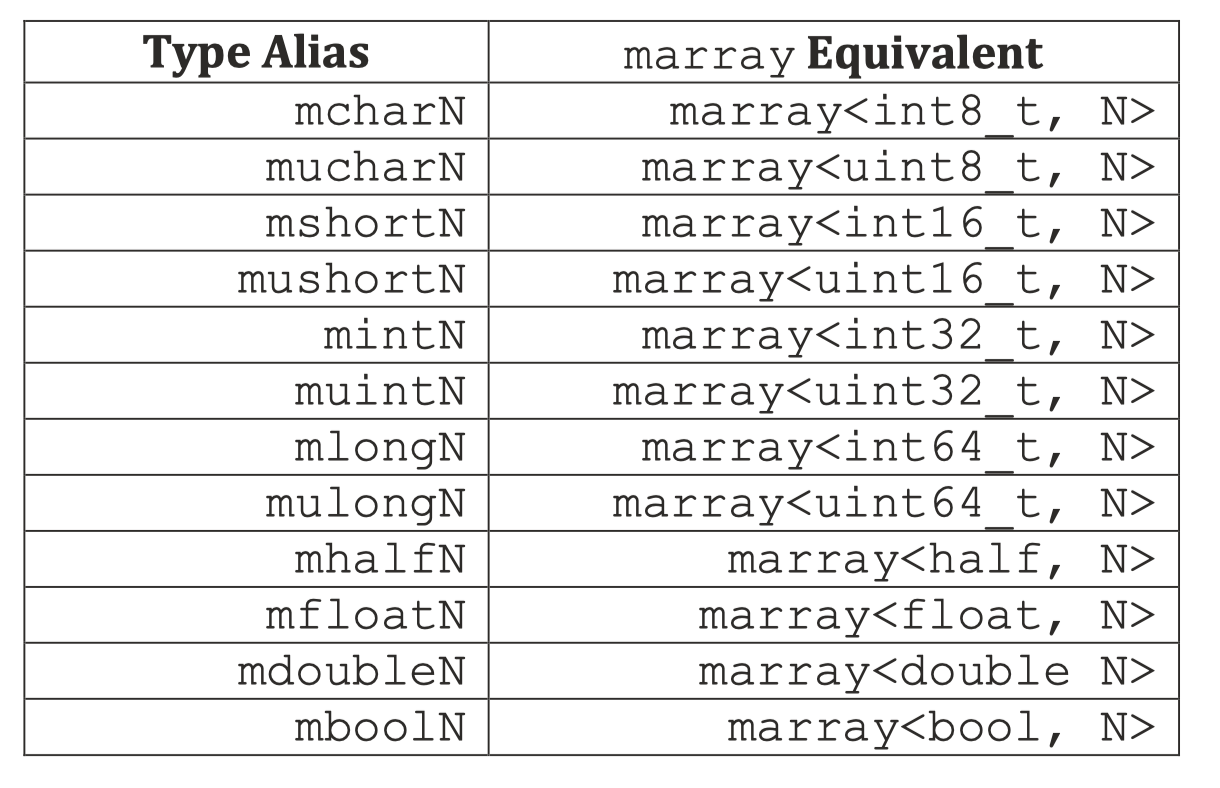
\includegraphics[width=0.9\textwidth]{figs/F11.1.png}
	\caption{\textit{基于加法的包容性扫描的简单顺序实现。}}
\end{figure}

在介绍并行扫描算法及其实现之前,我们想展示顺序包含扫描算法及其实现。 我们假设所涉及的运算符是加法。 
图 11.1 中的代码假设输入元素位于 $x$ 数组中,输出元素将写入 $y$ 数组中。

该代码使用输入元素 $x[0]$ 的值初始化输出元素 $y[0]$(第 02 行)。 
在循环的每次迭代中(第 03-05 行),循环体向前一个输出元素(存储所有先前输入元素的累加)添加一个输入元素,
以生成另一个输出元素。

应该清楚的是,图11.1中包含扫描的顺序实现所做的工作与输入元素的数量成线性比例; 即顺序算法的计算复杂度为$O(N)$。

在第 11.2-11.5 节中,我们将介绍执行并行分段扫描的替代算法,
其中每个线程块将对输入数组中的元素的一个段(即一个部分)执行并行扫描。 
然后,我们将在第 11.6 节和第 11.7 节中介绍将分段扫描结果组合到整个输入数组的扫描输出中的方法。

\subsection{使用 Kogge-Stone 算法进行并行扫描}
我们从简单的并行包含扫描算法开始,对每个输出元素执行归约操作。 
人们可能会想使用每个线程对一个输出元素执行顺序归约,如图 10.2 所示。 毕竟,这允许并行执行所有输出元素的计算。 
不幸的是,与图 11.1 中的顺序扫描代码相比,这种方法不太可能改善执行时间。 
这是因为 $y_{n-1}$ 的计算将采取 $n$ 步,与顺序扫描代码采取的步数相同,
并且归约中的每个步骤(迭代)涉及与每个步骤相同的工作量。 顺序扫描的迭代。 
由于并行程序的完成时间受到耗时最长的线程的限制,因此这种方法不太可能比顺序扫描更快。 
事实上,在计算资源有限的情况下,这种简单的并行扫描算法的执行时间可能比顺序算法的执行时间长得多。 
不幸的是,对于所提出的方法,计算成本或执行的操作总数会高得多。 
由于输出元素 $i$ 的归约步骤数为 $i$,因此所有线程执行的步骤总数为
$$
\sum_{i=0}^{n-1} i=\frac{n \cdot(n-1)}{2}
$$

也就是说,所提出的方法的计算复杂度为 $O\left(N^{2}\right)$,高于顺序扫描的复杂度,即 $O(N)$,同时没有提供加速 。 
计算复杂度越高意味着需要配置更多的执行资源。 这显然是一个坏主意。

更好的方法是采用第 10 章“归约和最小化散度”中的并行归约树,以使用相关输入元素的归约树来计算每个输出元素。 
有多种方法可以为每个输出元素设计归约树。 
由于元素$i$的归约树涉及$i$加法操作,这种方法仍然会将计算复杂度增加到$O\left(N^{2}\right)$,
除非我们找到一种方法来共享部分和 不同输出元素的归约树。 
我们提出了一种基于 Kogge-Stone 算法的共享方法,
该算法最初是在 20 世纪 70 年代为设计快速加法器电路而发明的(Kogge \& Stone,1973)。 
该算法至今仍在高速计算机运算硬件的设计中使用。 

\begin{figure}[H]
	\centering
	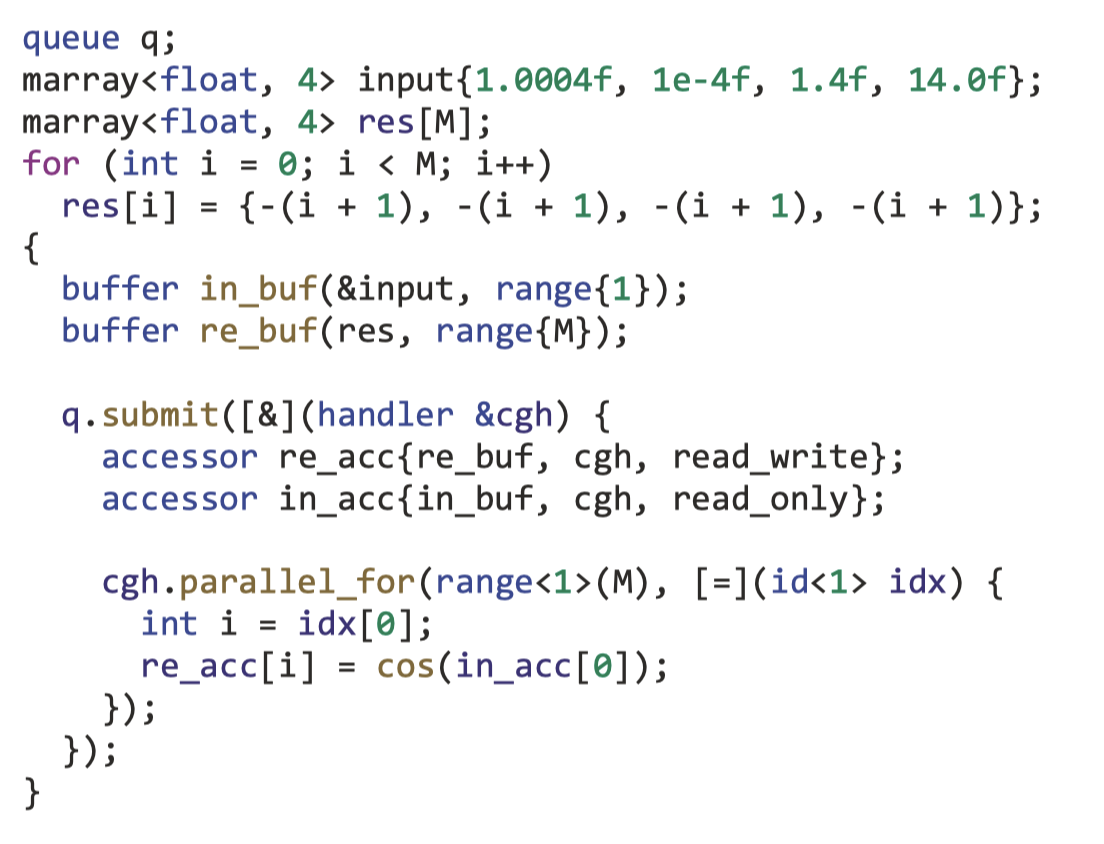
\includegraphics[width=0.9\textwidth]{figs/F11.2.png}
	\caption{\textit{基于Kogge-Stone加法设计的平行包含扫描算法。}}
\end{figure}

如图 11.2 所示,该算法是一种就地扫描算法,对最初包含输入元素的数组 XY 进行操作。 
它将数组的内容迭代地演变为输出元素。 在算法开始之前,我们假设 XY[i] 包含输入元素 $x_{i}$。 
经过 $k$ 次迭代后,$\mathrm{XY}$ [i] 将包含该位置及其之前最多 $2^{k}$ 个输入元素的总和。 
例如,在一次迭代之后,XY[i] 将包含 $x_{i-1}+x_{i}$,
在第 2 次迭代结束时,XY[i] 将包含 $x_{i-3}+x_{ i-2}+x_{i-1}+x_{i}$,依此类推。

图 11.2 以 16 元素输入示例说明了该算法。 每条垂直线代表 XY 数组的一个元素,其中 XY[0] 位于最左边的位置。 
垂直方向显示迭代的进度,从图的顶部开始。 对于包含式扫描,根据定义,$y_{0}$ 是 $x_{0}$,因此 XY[0] 包含其最终答案。 
在第一次迭代中,除 XY[0] 之外的每个位置接收其当前内容与其左邻居内容的总和。 图 11.2 中第一行加法运算符说明了这一点。 
结果,XY[i] 包含 $x_{i-1}+x_{i}$。 这反映在图 11.2 中第一行加法运算符下方的标签框中。 
例如,第一次迭代后,$X Y[3]$ 包含 $x_{2}+x_{3}$,
显示为 注意,第一次迭代后,$\mathrm{XY}[1]$ 等于 $ x_{0}+x_{1}$,这是该位置的最终答案。 
因此,在后续迭代中 XY[1] 不应再发生任何更改。

在第二次迭代中,除 XY[0] 和 XY[1] 之外的每个位置接收其当前内容与两个元素之外的位置的内容之和。 
这在第二行加法运算符下方的标记框中进行了说明。 结果,XY[i] 变为 $x_{i-3}+x_{i-2}+x_{i-1}+x_{i}$。 
例如,第二次迭代后,$\mathrm{XY}[3]$ 变为 $x_{0}+x_{1}+x_{2}+x_{3}$,显示为 $\sum x_{0} \ldots x_{3}$。 
请注意,第二次迭代后,$\mathrm{XY}[2]$ 和 $\mathrm{XY}[3]$ 已达到最终答案,在后续迭代中不需要更改。 
我们鼓励读者完成其余的迭代。

\begin{figure}[H]
	\centering
	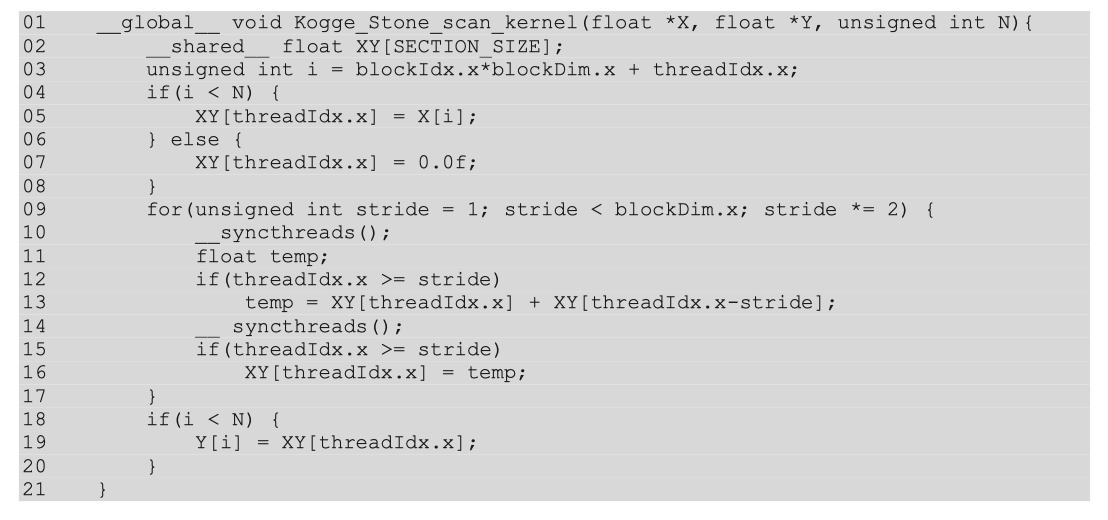
\includegraphics[width=0.9\textwidth]{figs/F11.3.png}
	\caption{\textit{用于包含(分段)扫描的 Kogge-Stone 内核。}}
\end{figure}

图 11.3 显示了图 11.2 所示算法的并行实现。 我们实现一个内核,对输入的不同段(部分)执行局部扫描,每个段都足够小,
可供单个块处理。 稍后,我们将进行最终调整,以合并大型输入阵列的这些截面扫描结果。 
节的大小定义为编译时常量 SECTION\_SIZE。 我们假设将使用 SECTION\_SIZE 作为块大小来调用内核函数,
因此将有相同数量的线程和节元素。 我们分配每个线程来演化一个 $\mathrm{XY}$ 元素的内容。

图 11.3 所示的实现假设输入值最初位于全局内存数组 $\mathrm{X}$ 中,其地址作为参数传递到内核(第 01 行)。 
我们将让块中的所有线程协作将 $\mathrm{X}$ 数组元素加载到共享内存数组 XY 中(第 02 行)。 
这是通过让每个线程计算其全局数据索引 i=blockIdx.x * blockDim.x+threadIdx.x(第03行)为其负责的输出向量元素位置来实现的。 
每个线程将该位置的输入元素加载到内核开头的共享内存中(第 04-08 行)。
在内核结束时,每个线程会将其结果写入指定的输出数组 Y(第 18-20 行)。

我们现在重点关注图 11.3 中每个 $\mathrm{XY}$ 元素作为 for 循环的迭代计算的实现(第 09-17 行)。 
该循环迭代归约树以找到分配给线程的 $\mathrm{XY}$ 数组位置。 当步幅值大于线程的 threadIdx 时。 
$x$ 值,这意味着线程分配的 XY 位置已经累积了所有所需的输入值,并且线程不再需要处于活动状态(第 12 和 15 行)。 
请注意,我们使用屏障同步(第 10 行)来确保所有线程在任何线程开始下一次迭代之前都已完成其上一次迭代。 
这与第 10 章“减少和最小化发散”中的减少讨论中 \_syncthreads() 的使用相同。

然而,与 for 循环每次迭代中 XY 元素更新(第 12-16 行)的减少相比,存在非常重要的差异。 
请注意,每个活动线程首先将其位置的部分和存储到临时变量(在寄存器中)中。 
所有线程完成第二次屏障同步后(第 14 行),所有线程都将其部分和值存储到其 $\mathrm{XY}$ 位置(第 16 行)。 
对额外 temp 和 \_\_syncthreads() 的需求与这些更新中的读后写数据依赖危险有关。 
每个活动线程在其自己的位置 (XY[threadIdX.X]) 和另一个线程的位置 (XY[threadIdX.X-stride]) 处添加 $X Y$ 值。 
如果线程 $i$ 在另一个线程 i+stride 有机会读取该位置的旧值之前写入其输出位置,则新值可能会破坏另一个线程执行的加法。 
损坏可能发生也可能不发生,具体取决于所涉及线程的执行时间,这称为竞争条件。 
请注意,这种竞争条件与我们在第 9 章“并行直方图”中看到的直方图模式不同。 
第 9 章“并行直方图”中的竞争条件是读取-修改-写入竞争条件,可以通过原子操作来解决。 
对于我们在这里看到的读后写竞争条件,需要不同的解决方案。

在图 11.2 中可以很容易地观察到竞争条件。 
让我们检查迭代 2 期间线程 $4\left(x_{4}\right)$ 和线程 $6\left(x_{6}\right)$ 的活动,这表示为从 顶部。 
请注意,线程 6 需要将 XY[4] $(x_{3}+x_{4})$ 的旧值添加到旧值 XY[6] $(x_{5}+x_ {6})$ 
生成 XY[6] $(x_{3}+x_{4}+x_{5}+x_{6})$ 的新值。 
但是,如果线程 4 过早地将迭代 $(x_{1}+x_{2}+x_{3}+x_{4})$ 的加法结果存储到 XY[4] 中,
则线程 6 可能会 最终使用新值作为输入并将 $(x_{1}+x_{2}+x_{3}+x_{4}+x_{5}+x_{6})$ 存储到 $ \mathrm{XY}[6]$。 
由于 $x_{1}+x_{2}$ 将在第三次迭代中由线程 6 再次添加到 XY[6],
因此 XY[6] 中的最终答案将变为 $(2 x_{1}+2 x_{2}+x_{3}+x_{4}+x_{5}+x_{6})$,这显然是不正确的。 
另一方面,如果线程 6 在迭代 2 期间线程 4 覆盖 XY[4] 中的旧值之前恰好读取了旧值,则结果将是正确的。 
也就是说,代码的执行结果可能正确也可能不正确,具体取决于线程执行的时间,并且每次运行的执行结果可能会有所不同。 
这种可重复性的缺乏会使调试成为一场噩梦。

第 13 行中使用的临时变量和第 14 行中的 \_syncthreads () 屏障克服了竞争条件。
在第 13 行中,所有活动线程首先执行加法并写入其私有临时变量。 因此,XY 位置中的任何旧值都不会被覆盖。 
第 14 行中的屏障 \_syncthread() 确保所有活动线程都已完成对旧 XY 值的读取,然后才能向前移动并执行写入。 
因此,第 16 行中的语句覆盖 XY 位置是安全的。

更新的 XY 位置可以由另一个活动线程使用的原因是 Kogge-Stone 方法在归约树中重用部分和以降低计算复杂性。 
我们将在 11.3 节中进一步研究这一点。 
读者可能想知道为什么第 10 章“减少和最小化发散”中的减少树内核不需要使用临时变量和额外的 \_syncthreads()。 
答案是,这些归约内核中不存在由读后写危险引起的竞争条件。 
这是因为迭代中活动线程写入的元素在同一迭代期间不会被任何其他活动线程读取。 
通过检查图 10.7 和 10.8 应该可以看出这一点。 
例如,在图 10.8 中,每个活动线程从其自己的位置(输入 [threadIdx.x])和向右跨距的位置(输入 [threadIdx.x+stride])获取输入。 在任何给定迭代期间,任何活动线程都不会更新任何步幅距离位置。 
因此,所有活动线程始终能够读取其各自输入[threadIdx.x]的旧值。 
由于线程内的执行始终是顺序的,因此每个线程始终能够在将新值写入该位置之前读取 input[threadIdx.x] 中的旧值。 
读者应该验证图 10.7 中是否存在相同的属性。

如果我们想避免在每次迭代时出现第二次屏障同步,克服竞争条件的另一种方法是对输入和输出使用单独的数组。 
如果使用单独的数组,则写入的位置与读取的位置不同,因此不再存在任何潜在的读后写入竞争条件。 
这种方法需要有两个共享内存缓冲区而不是一个。 首先,我们从全局内存加载到第一个缓冲区。 
在第一次迭代中,我们从第一个缓冲区读取并写入第二个缓冲区。 
迭代结束后,第二个缓冲区中有最新的结果,第一个缓冲区中的结果不再需要。 
因此,在第二次迭代中,我们从第二个缓冲区读取并写入第一个缓冲区。 
遵循相同的推理,在第三次迭代中,我们从第一个缓冲区读取并写入第二个缓冲区。 我们继续交替输入/输出缓冲区,直到迭代完成。 
这种优化称为双缓冲。 双缓冲通常用于并行编程中,作为克服读后写竞争条件的一种方法。 我们将这种优化的实现留给读者作为练习。 

此外,如图11.2所示,$\mathrm{XY}$较小位置上的动作比较大位置上的动作更早结束(参见if语句条件)。 
当步幅值较小时,这将导致第一个warp中出现一定程度的控制发散。 请注意,相邻线程往往会执行相同数量的迭代。 
对于大块大小,发散的影响应该相当适度,因为发散只会在第一个warp中出现。 详细分析留给读者作为练习。

\begin{figure}[H]
	\centering
	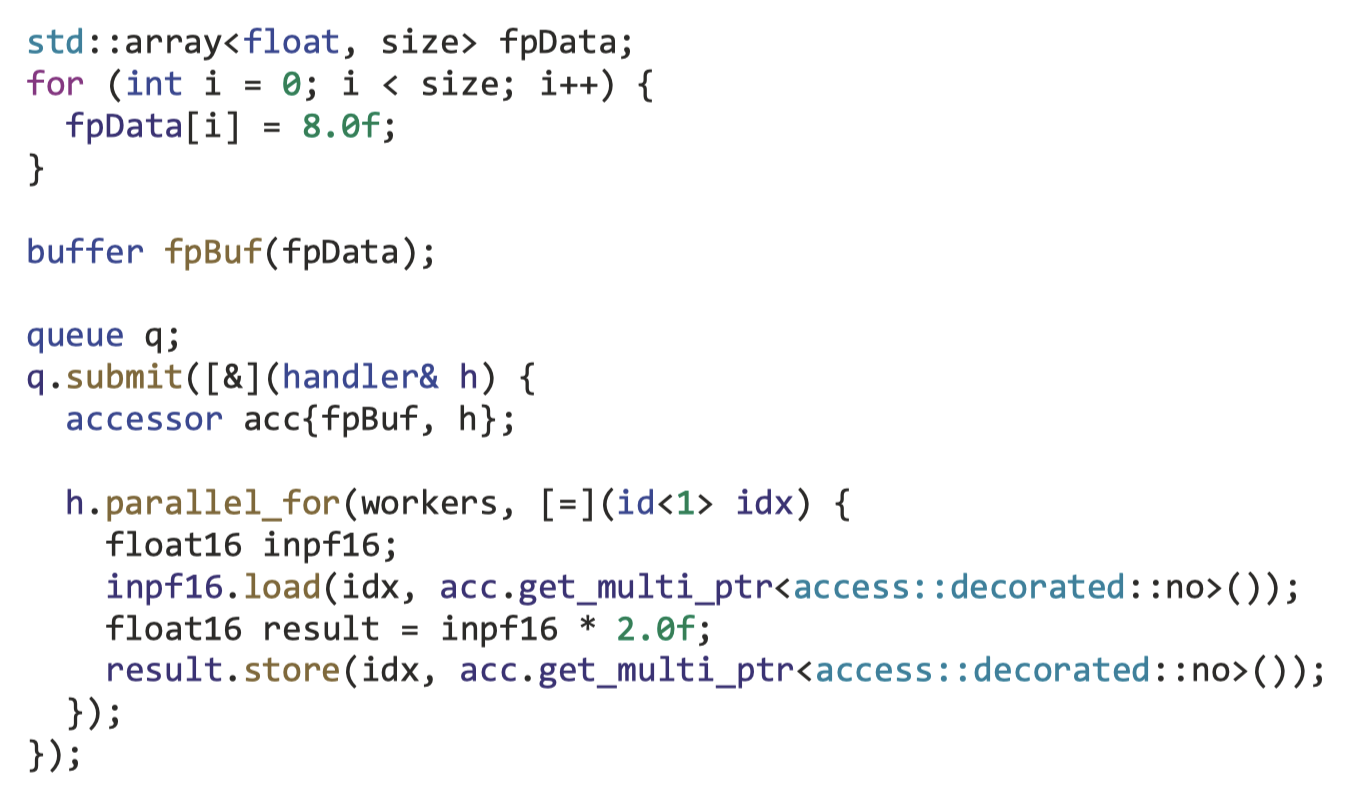
\includegraphics[width=0.9\textwidth]{figs/F11.4.png}
	\caption{\textit{一种基于Kogge-Stone加法器设计的并行独占扫描算法。}}
\end{figure}

虽然我们只展示了包含扫描内核,但我们可以轻松地将包含扫描内核转换为排除扫描内核。 
回想一下,排除扫描相当于包含扫描,其中所有元素向右移动一个位置,并且元素 0 填充标识值。 如图 11.4 所示。 
请注意,唯一真正的区别是图片顶部元素的对齐方式。 所有标签框均已更新以反映新的对齐方式。 所有迭代操作保持不变。

我们现在可以轻松地将图 11.3 中的内核转换为排除扫描内核。 
我们唯一需要做的修改就是将 0 加载到 XY[0] 中,将 $X[i-1]$ 加载到 $XY[$threadIdx.X] 中,如以下代码所示:

\begin{figure}[H]
	\centering
	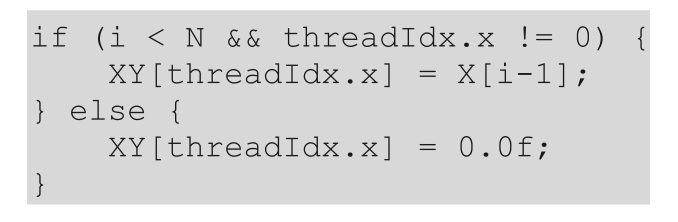
\includegraphics[width=0.9\textwidth]{figs/F11-a1.png}
\end{figure}

通过用这四行代码替换图 11.3 中的 04-08 行,我们将包含扫描内核转换为排除扫描内核。 
我们把完成排除扫描内核的工作留给读者作为练习。

\subsection{速度和工作效率的考虑}
分析并行算法的一个重要考虑因素是工作效率。 算法的工作效率是指算法执行的工作量接近计算所需的最小工作量的程度。 
例如,扫描操作所需的最小加法次数为$N-1$次加法,或$O(N)$,这是顺序算法执行的加法次数。 
然而,正如我们在第 11.2 节开头所看到的,朴素并行算法执行 $N^{*}(N-1) / 2$ 加法,或 $O$ $\left(N^{2}\right)$ ,
它比顺序算法大得多。 因此,简单的并行算法工作效率不高。

我们现在分析图11.3中Kogge-Stone内核的工作效率,重点关注单个线程块的工作。 
所有线程迭代最多 $\log _{2} N$ 步,其中 $N$ 是 SECTION\_SIZE。 在每次迭代中,非活动线程的数量等于步幅大小。 
因此,我们可以计算算法完成的工作量(for 循环的一次迭代,由图 8.1 中的加操作表示):
$$
\sum_{\text {stride }}(N-\text { stride }), \text { for strides } 1,2,4, \ldots N / 2\left(\log_{2} N \text { terms }\right)
$$

每一项的第一部分与步幅无关,其总和总计为 $N^{*} \log _{2}(N)$。 
第二部分是熟悉的几何级数,总计为$(N-1)$。 所以,完成的总工作量是
$$
N^{*} \log _{2}(N)-(N-1)
$$

好消息是 Kogge-Stone 方法的计算复杂度为 $O\left(N^{*} \log _{2}(N)\right)$,
优于 $O\left(N^{ 2}\right)$ 对所有输出元素执行完整归约树的简单方法的复杂性。 
坏消息是 Kogge-Stone 算法的工作效率仍然不如顺序算法。 
即使对于中等大小的部分,图 11.3 中的内核也会比顺序算法做更多的工作。 
在 512 个元素的情况下,内核执行的工作量大约是顺序代码的八倍。 该比率将随着 $N$ 变大而增加。

尽管 Kogge-Stone 算法比顺序算法执行更多的计算,但由于并行执行,它的步骤更少。 
顺序代码的 for 循环执行 $N$ 次迭代。 对于内核代码,每个线程的for循环最多执行$\log _{2} \mathrm{~N}$迭代,
它定义了执行内核所需的最少步骤数。 
在执行资源不受限制的情况下,内核代码相对于顺序代码的步骤数减少大约为 $N / \log _{2}(N)$。 
对于 $N=512$,步数减少约为 $512/9=56.9\times$ 。

在真实的 CUDA GPU 设备中,Kogge-Stone 内核完成的工作量比理论上的 $N^{*} \log 2(N)-(N-1)$ 还要多。 
这是因为我们正在使用 $N$ 线程。 
虽然许多线程停止参与for循环的执行,但其中一些线程仍然消耗执行资源,直到整个warp完成执行。 
实际上,Kogge-Stone 消耗的执行资源量更接近 $N^{*} \log 2(N)$。

我们将使用计算步骤的概念作为比较扫描算法的近似指标。 顺序扫描大约需要 $N$ 个步骤来处理 $N$ 个输入元素。 
例如,顺序扫描应采取大约 1024 个步骤来处理 1024 个输入元素。 
通过 CUDA 设备中的 $P$ 执行单元,我们可以预期 Kogge-Stone 内核执行 $\left(N^{*} \log 2(N)\right) / P$ 步骤。 
如果$P$等于$N$,也就是说,如果我们有足够的执行单元来并行处理所有输入元素,那么我们需要$\log 2(N)$步骤,
正如我们之前看到的。 然而,$P$ 可能小于 $N$。 
例如,如果我们使用 1024 个线程和 32 个执行单元来处理 1024 个输入元素,
内核可能会执行 $\left(1024^{*} 10\right) / 32=320$ 步骤。 
在这种情况下,我们预计步骤数将减少 $1024 / 320=3.2 \times$。

Kogge-Stone 内核在顺序代码上完成的额外工作在两个方面存在问题。 首先,使用硬件来执行并行内核的效率要低得多。 
如果硬件没有足够的资源(即,如果 $P$ 很小),则并行算法最终可能比顺序算法需要更多的步骤。 因此并行算法会更慢。 
其次,所有额外的工作都会消耗额外的能量。 这使得内核不太适合功耗受限的环境,例如移动应用程序。

Kogge-Stone内核的优势在于,当有足够的硬件资源时,它可以达到非常好的执行速度。 
它通常用于计算具有适度数量元素(例如 512 或 1024)的部分的扫描结果。
当然,这是假设 GPU 可以提供足够的硬件资源并使用额外的并行性来容忍延迟。 正如我们所看到的,其执行的控制发散量非常有限。 
在较新的 GPU 架构中,可以通过 warps 内的 shuffle 指令有效地执行计算。 
我们将在本章后面看到它是现代高速并行扫描算法的重要组成部分。

\subsection{使用 Brent-Kung 算法进行并行扫描}
虽然图11.3中的Kogge-Stone内核在概念上很简单,但对于某些实际应用来说,其工作效率相当低。 
只需检查图 11.2和11.4,我们可以看到一些中间结果有进一步共享的潜在机会。 
然而,为了允许跨多个线程更多地共享,我们需要策略性地计算中间结果并将它们分发到不同的线程,这可能需要额外的计算步骤。

众所周知,为一组值生成总和的最快并行方法是归约树。 
有了足够的执行单元,归约树可以在 $\log_{2}(N)$ 时间单位内生成 $N$ 值的总和。 
该树还可以生成多个子和,这些子和可用于计算某些扫描输出值。 
这一观察结果被用作 Kogge-Stone 加法器设计的基础,
也构成了 Brent-Kung 加法器设计的基础(Brent \& Kung,1979)。 
Brent-Kung加法器设计还可用于实现并行扫描算法,工作效率更好。

\begin{figure}[H]
	\centering
	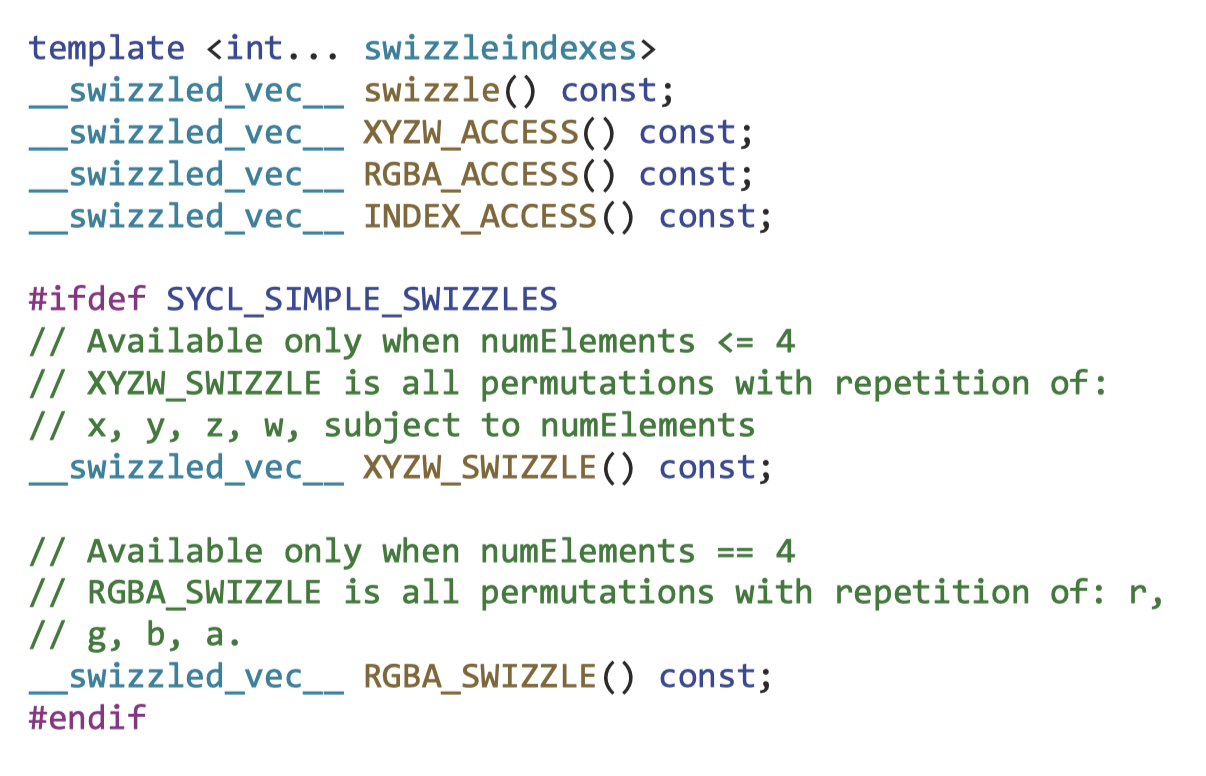
\includegraphics[width=0.9\textwidth]{figs/F11.5.png}
	\caption{\textit{一种基于Brent-Kung加法器设计的并行包含扫描算法。}}
\end{figure}

图 11.5 说明了基于 Brent-Kung 加法器设计的并行包含扫描算法的步骤。 
在图 11.5 的上半部分,我们分四步计算所有 16 个元素的总和。 我们使用生成总和所需的最少操作数。 
在第一步中,只有 XY[i] 的奇数元素会更新为 XY[i-1] $+\mathrm{XY}[\mathrm{i}]$。 
在第二步中,仅更新索引为$4^{*} n-1$形式的XY元素,即图11.5中的3、7、11和15。 
在第三步中,只有索引为 $8^{*} n-1$ 形式(即 7 和 15 )的 XY 元素才会被更新。 
最后,在第四步中,仅更新 XY[15]。 执行的操作总数为$8+4+2+1=15$。 
一般来说,对于 $N$ 个元素的扫描部分,我们会在这个归约阶段执行 $(N / 2)+(N / 4)+\ldots+2+1=N-1$ 操作。

该算法的第二部分是使用反向树将部分和分配到可以使用它们来完成这些位置的结果的位置。 
部分和的分布如图 11.5 的下半部分所示。 为了理解反向树的设计,我们首先应该分析一下需要额外的值来完成XY每个位置的扫描输出。 
从图 11.5 中可以明显看出,归约树中的添加总是在连续范围内累积输入元素。 
因此我们知道,已经累积到 XY 每个位置的值总是可以表示为输入元素 $x_{i} \ldots x_{j}$ 的范围,
其中 $x_{i}$ 是起始位置, $x_{j}$ 是结束位置(包含)。

\begin{figure}[H]
	\centering
	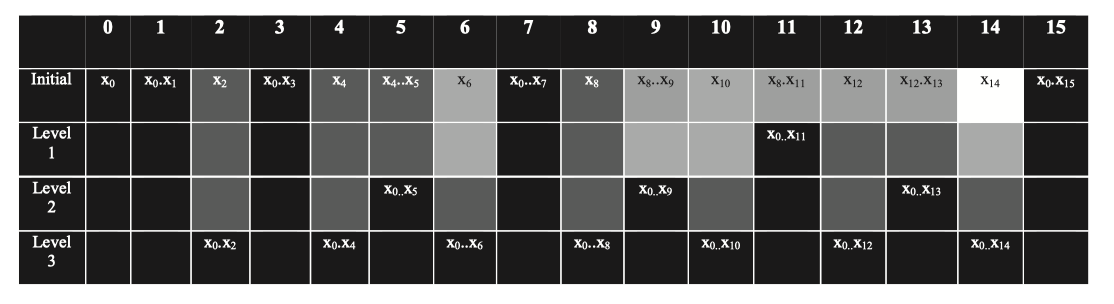
\includegraphics[width=0.9\textwidth]{figs/F11.6.png}
	\caption{\textit{在反向树中每一级求和之后,XY 中的值的变化。}}
\end{figure}

图11.6显示了每个位置(列)的状态,包括已经累积到该位置的值以及反向树的每个级别(行)需要额外的输入元素值。 
反向树中最初和每级添加之后的每个位置的状态表示为输入元素,其形式为 $x_{i} \ldots x_{j}$,这些元素已在该位置中考虑。 
例如,第 11 行、第 11 列中的 $x_{8} \ldots x_{11}$ 表示 $x_{8}、x_{9}、x_{10}$ 和 $x_{11}$ 的值,
在反向树开始之前(就在图 11.5 底部所示的归约阶段之后),已经累积到 $\mathrm{XY}[11]$ 中。 
在归约树阶段结束时,我们有相当多的位置完成了最终的扫描值。 
在我们的示例中,XY[0]、XY[1]、$\mathrm{XY}[3]$、$\mathrm{XY}[7]$ 和 $\mathrm{XY}[15]$ 都得到了最终的答案。

需要额外的输入元素值由图 11.6 中每个单元格的阴影表示:白色表示该位置需要从其他三个位置累加部分和,
浅灰色表示 2,深灰色表示 1,黑色表示 0。 
例如,最初,XY[14] 被标记为白色,因为它在归约树阶段结束时只有 $x_{14}$ 的值,
并且需要累加 XY[7] $\left(x_ {0} \ldots x_{7}\right)、\mathrm{XY}[11]\left(x_{8} \ldots x_{11}\right)$ 
和 $\mathrm{XY}[13]\left(x_{12} \ldots x_{13}\right)$ 
完成其最终扫描值$\left(x_{0} \ldots x_{14}\right)$。 
读者应该验证,由于归约树的结构,
大小为 $N$ 元素的输入的 XY 位置将永远不需要来自超过 $\log _{2}(N)-1$ 部分和的累加 其他 XY 位置。 
此外,这些部分总和位置彼此之间的距离始终为 $1,2,4, \ldots$(2 的幂)。 
在我们的示例中,XY[14] 需要 $\log _{2}(16)-1=3$ 来自位置 1($X Y[14]$ 和 $X Y$ [13] 之间)的部分和,
2 ( XY[13] 和 XY[11] 之间)和 4(XY[11] 和 XY[7] 之间)。

为了组织加法运算的后半部分,我们将首先展示所有需要从四个位置之外进行部分求和的运算,然后是两个位置之外,然后是一个位置之外。 
在反向树的第一层中,我们将 XY[7] 添加到 XY[11],这将 XY[11] 带到最终答案。 
在图 11.6 中,位置 11 是唯一进入最终答案的位置。 
在第二级中,我们完成 XY[5]、XY[9] 和 XY[13],
这可以用两个位置之外的部分和来完成: $\mathrm{XY}[3], \mathrm{ 分别为 XY}[7]$ 和 $\mathrm{XY}[11]$。 
最后,在第三级中,我们通过累加部分和来完成所有偶数位置 $X Y$ [2]、XY[4]、XY [6]、XY[8]、XY[10] 和 XY[12] 相距一个位置(每个位置的左邻)。

我们现在准备实施 Brent-Kung 扫描方法。 我们可以使用以下循环来实现并行扫描的归约树阶段:

\begin{figure}[H]
	\centering
	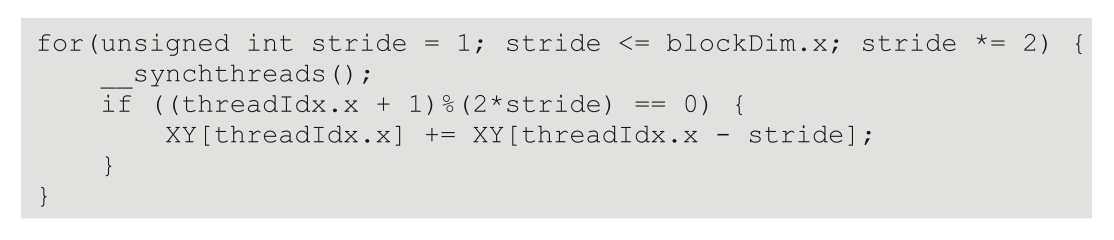
\includegraphics[width=0.9\textwidth]{figs/F11-a2.png}
\end{figure}

请注意,该循环与图 10.6 中的归约类似。 只有两点不同。 第一个区别是我们将总和值向最高位置累积,即 XY[blockDim.X-1],
而不是 XY[0]。 这是因为最高位的最终结果就是总和。 因此,每个活动线程通过从其索引中减去步幅值来获得其左侧的部分总和。 
第二个区别是我们希望活动线程具有 $2^{n}-1$ 形式的线程索引,而不是 $2^{n}$。 
这就是为什么每次迭代中选择执行加法的线程时,我们在取模(\%)运算之前将 threadIdx.x 加 1。

这种归约方式的一个缺点是它具有严重的控制发散问题。 正如我们在第 10 章“减少和最小化发散”中看到的,
更好的方法是随着循环的进行,使用数量不断减少的连续线程来执行加法。 
不幸的是,我们在图 10.8 中用来减少发散的技术不能在扫描归约树阶段使用,
因为它不会在中间 $\mathrm{XY}$ 位置生成所需的部分和值。 
因此,我们采用更复杂的线程索引到数据索引映射,将线程的连续部分映射到一系列相距一定距离的数据位置。 
以下代码通过将线程的连续部分映射到索引格式为 $k^{*} 2^{n}-1$ 的 XY 位置来实现此目的:

\begin{figure}[H]
	\centering
	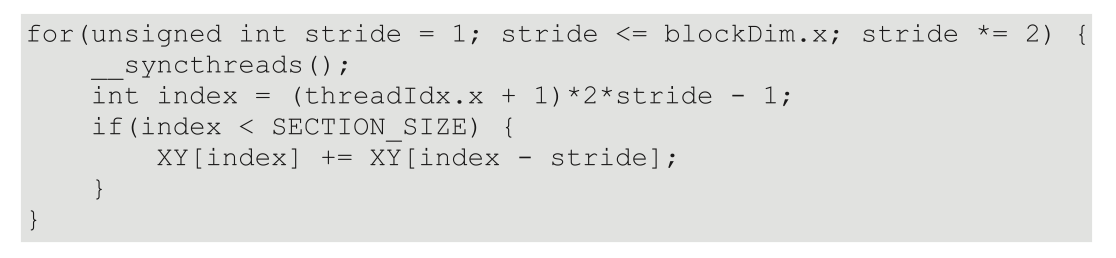
\includegraphics[width=0.9\textwidth]{figs/F11-a3.png}
\end{figure}

通过在 for 循环的每次迭代中使用如此复杂的索引计算,每次迭代中将使用从线程 0 开始的一组连续线程,以避免warp内的控制发散。 
在图 11.5 的小示例中,块中有 16 个线程。 在第一次迭代中,步幅等于 1 。 块中的前八个连续线程将满足 if 条件。 
为这些线程计算的 XY 索引值将为 $1,3,5,7,9,11,13$ 和 15 。 这些线程将执行图 11.5 中的第一行添加。 
在第二次迭代中,步长等于 2。只有块中的前四个线程才会满足 if 条件。 为这些线程计算的索引值将为 $3,7,11$ 和 15 。 
这些线程将执行图 11.5 中的第二行添加。 
请注意,由于每次迭代始终使用连续的线程,因此在活动线程数降至warp大小以下之前,不会出现控制发散问题。

反向树的实现稍微复杂一些。 我们看到步幅值从 SECTION\_SIZE/4 减小到 1 。 
在每次迭代中,我们需要将 XY 元素的值从步幅值减 1 的两倍的位置向右“推”步幅位置。 
例如,在图 11.5 中,步幅值从 $4\left(2^{2}\right)$ 减小到 1 。 
在第一次迭代中,我们希望将 XY[7] 的值推(添加)到 XY[11] 中,其中 7 是 $2^{*} 2^{2}-1$,
距离(步幅)是 $2^{ 2}$。 请注意,只有线程 0 将用于此迭代,因为为其他线程计算的索引太大而无法满足 if 条件。 
在第二次迭代中,我们将 XY[3]、XY[7] 和 XY[11] 的值分别推入 XY[5]、XY[9] 和 XY[13]。 
索引 3,7 和 11 分别为 $1^{*} 2^{*} 2^{1}-1,2^{*} 2^{*} 2^{1}-1$ 和 $3^{*} 2^{*} 2^{1}-1$。 
目标位置距离源位置为 $2^{1}$ 个位置。 
最后,在第三次迭代中,我们将所有奇数位置的值推送到其偶数位置右侧邻居 $\left(\right.$ stride $=2^{\circ}$ )。

在上述讨论的基础上,反向树可以通过以下循环来实现:

\begin{figure}[H]
	\centering
	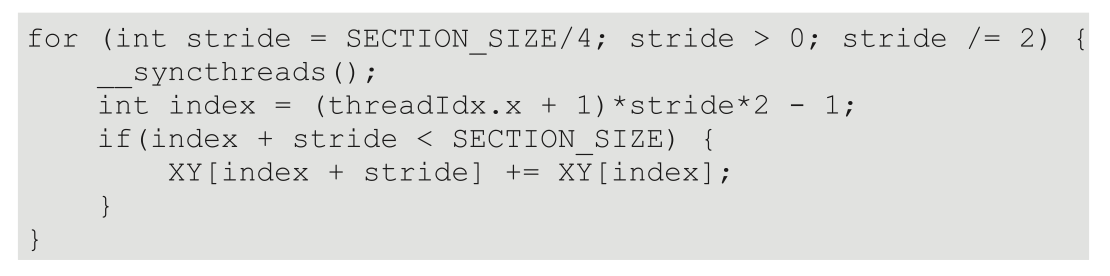
\includegraphics[width=0.9\textwidth]{figs/F11-a4.png}
\end{figure}

索引的计算与归约树阶段类似。 $X Y$ [index+stride] +=XY[indeX] 语句反映了从线程的映射位置推送到跨步的更高位置。

\begin{figure}[H]
	\centering
	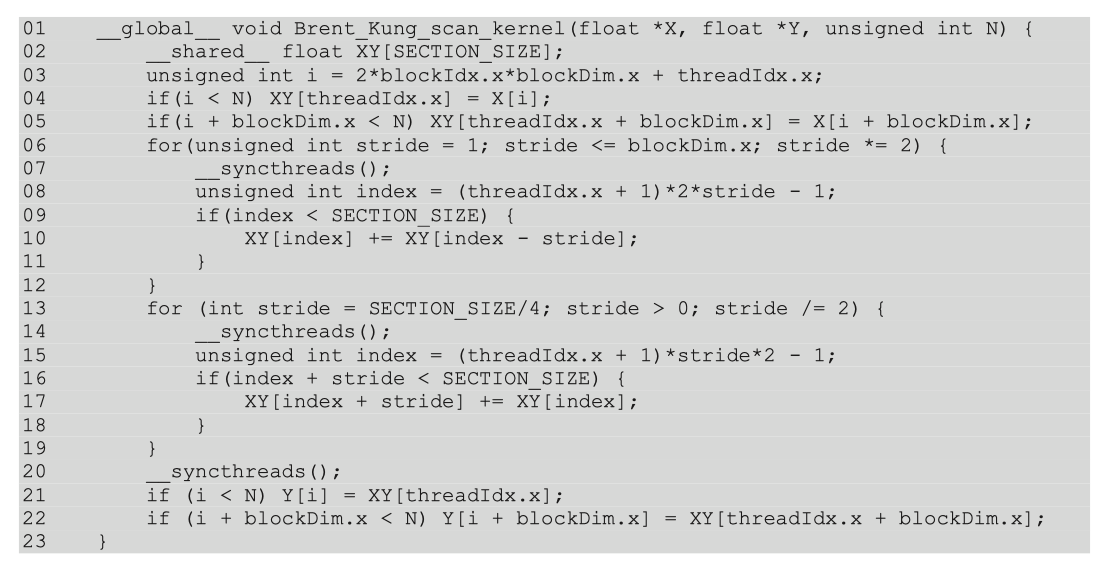
\includegraphics[width=0.9\textwidth]{figs/F11.7.png}
	\caption{\textit{用于包含(分段)扫描的 Brent-Kung 内核。}}
\end{figure}

Brent-Kung 并行扫描的最终内核代码如图 11.7 所示。 
读者应该注意到,对于归约阶段或分发阶段,我们永远不需要超过 SECTION\_SIZE/2 的线程。 
因此,我们可以简单地启动一个块中包含 SECTION\_SIZE/2 个线程的内核。 
由于块中最多可以有 1024 个线程,因此每个扫描部分最多可以有 2048 个元素。 
但是,我们需要让每个线程在开头加载两个 X 元素,并在末尾存储两个 Y 元素。

与 Kogge-Stone 扫描内核的情况一样,只需对将 X 元素加载到 XY 的语句进行细微调整,
就可以轻松地将 Brent-Kung 包含并行扫描内核改编为排除扫描内核。 有兴趣的读者还应该阅读 Harris et al., 2007,
了解一个有趣的本机独有的扫描内核,该内核基于设计扫描内核的反向树阶段的不同方式。

现在我们将注意力转向反向树阶段操作数的分析。 运算次数为$(16 / 8)-1+(16 / 4)-1+(16 / 2)-1$。 
一般来说,对于 $N$ 个输入元素,操作总数为 $(2-1)$ $+(4-1)+\ldots+(N / 4-1)+(N / 2-1)$, 
即 $N-1-\log _{2}(N)$。 因此并行扫描中的操作总数,
包括归约树 $(N-1$ 操作) 和逆向树 $\left(N-1-\log _{2}(N)\right.$ 操作 ) 阶段,为 $2^{*} N-2-\log _{2}(N)$。 
请注意,操作总数现在为 $O(N)$,而不是 Kogge-Stone 算法的 $O\left(N^{*} \log _{2} N\right)$。

Brent-Kung 算法相对于 Kogge-Stone 算法的优势非常明显。 
随着输入部分变大,Brent-Kung 算法执行的操作数永远不会超过顺序算法执行的操作数的 2 倍。 
在能量受限的执行环境中,Brent-Kung 算法在并行性和效率之间取得了良好的平衡。

虽然Brent-Kung算法比Kogge-Stone算法具有更高水平的理论工作效率,但其在CUDA内核实现中的优势更为有限。 
回想一下,Brent-Kung 算法使用 N/2 个线程。 主要区别在于,通过归约树,活动线程数量下降的速度比 Kogge-Stone 算法快得多。 
然而,一些不活动线程可能仍然消耗 CUDA 设备中的执行资源,因为它们通过 SIMD 绑定到其他活动线程。 
这使得在 CUDA 设备中 Brent-Kung 相对于 Kogge-Stone 的工作效率优势不那么明显。

与 Kogge-Stone 相比,Brent-Kung 的主要缺点是尽管工作效率更高,但执行时间可能更长。 
凭借无限的执行资源,Brent-Kung 的时间大约是 Kogge-Stone 的两倍,因为需要额外的步骤来执行反向树阶段。 
然而,当我们的执行资源有限时,速度比较可能会有很大不同。 
使用第 11.3 节中的示例,如果我们使用 32 个执行单元处理 1024 个输入元素,
则 Brent-Kung 内核预计将执行大约 $(2 * 1024-2-10) / 32=63.6$ 步。 
读者应该验证,在控制发散的情况下,当每个阶段的活动线程总数降至 32 以下时,还会有大约 5 个步骤。 
与顺序执行相比,这会带来 1024/73.6=14 的加速。 与 Kogge-Stone 的 320 个时间单位和 3.2 的加速相比。 
当然,当执行资源更多和/或延迟更长时,这种比较将具有 Kogge-Stone 的优势。

\subsection{粗化以提高效率}
跨多个线程并行扫描的开销就像减少一样,因为它包括硬件未充分利用和树执行模式的同步开销。 
然而,扫描有额外的并行化开销,这会降低工作效率。 正如我们所看到的,并行扫描的工作效率低于顺序扫描。 
如果线程实际上是并行运行的,那么较低的工作效率是可以接受的并行化代价。 
但是,如果硬件要序列化它们,我们最好自己通过线程粗化来序列化它们,以提高工作效率。

我们可以设计一种并行分段扫描算法,通过在输入的各个分段上添加一个完全独立的顺序扫描阶段来实现更好的工作效率。 
每个线程块接收比原始部分大粗化因子的输入部分。 
在算法开始时,我们将输入的块部分划分为多个连续的子部分:每个线程一个子部分。 分段的数量与线程块中线程的数量相同。

\begin{figure}[H]
	\centering
	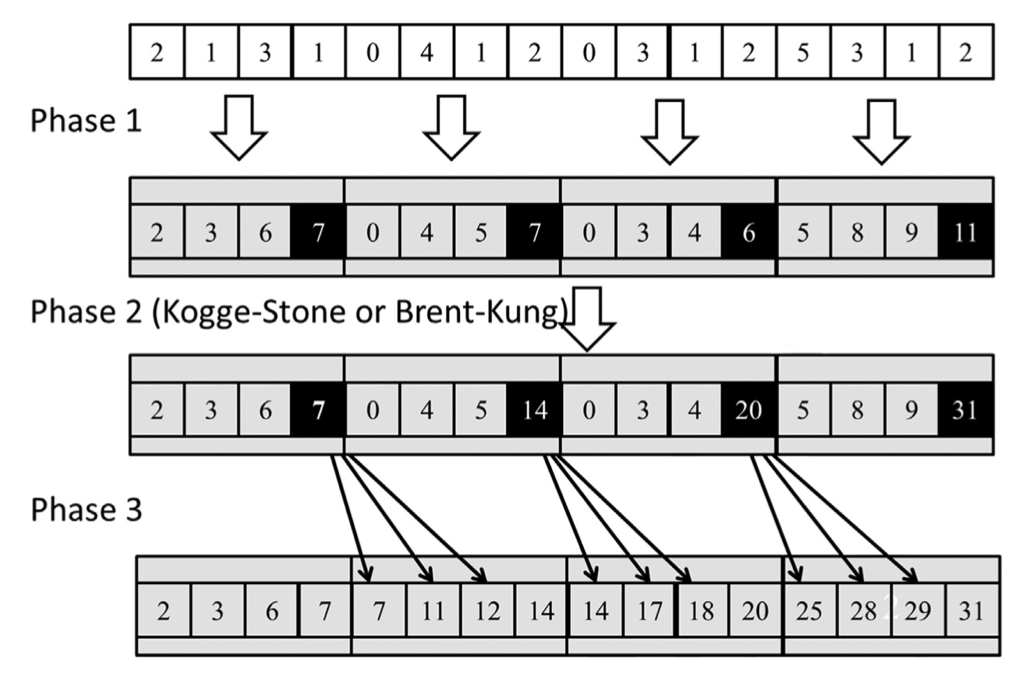
\includegraphics[width=0.9\textwidth]{figs/F11.8.png}
	\caption{\textit{工作效率更高的三阶段并行扫描。}}
\end{figure}

粗化扫描分为三个阶段,如图 11.8 所示。 在第一阶段,我们让每个线程对其连续的分段执行顺序扫描。 
例如,在图 11.8 中,我们假设一个块中有四个线程。 我们将 16 个元素的输入部分分为四个子部分,每个子部分有四个元素。 
线程0将对其部分$(2,1,3,1)$执行扫描并生成$(2,3,6,7)$。 
线程1将对其部分$(0,4,1,2)$执行扫描并生成$(0,4,5,7)$,依此类推。

请注意,如果每个线程直接通过访问全局内存中的输入来执行扫描,则它们的访问将不会合并。 
例如,在第一次迭代期间,线程 0 将访问输入元素 0 ,线程 1 将访问输入元素 4 ,依此类推。 
因此,我们通过使用共享内存来吸收无法合并的内存访问来改进内存合并,如第 6 章“性能注意事项”中提到的。 
也就是说,我们以合并的方式在共享内存和全局内存之间传输数据,并在共享内存中以不利的访问模式执行内存访问。 
在第一阶段开始时,所有线程协作以迭代方式将输入加载到共享内存中。 在每次迭代中,相邻线程加载相邻元素以启用内存合并。 
例如,在图 11.8 中,我们让所有线程协作并以合并的方式加载四个元素:线程 0 加载元素 0 ,线程 1 加载元素 1 ,依此类推。 
然后,所有线程都会移动以加载接下来的四个元素:线程 0 加载元素 4 ,线程 1 加载元素 5 ,依此类推。

一旦所有输入元素都位于共享内存中,线程就会从共享内存中访问自己的子部分并对其执行顺序扫描。 这如图 11.8 中的阶段 1 所示。 
请注意,在第 1 阶段结束时,每个部分的最后一个元素(在第二行中突出显示为黑色)包含该部分中所有输入元素的总和。 
例如,第 0 节的最后一个元素包含值 7 ,即该节中输入元素 $(2,1,3,1)$ 的总和。

在第二阶段,每个块中的所有线程协作并对由每个部分的最后一个元素组成的逻辑数组执行扫描操作。 
这可以通过 Kogge-Stone 或 Brent-Kung 算法来完成,因为只有适量的元素(块中的线程数)。 
请注意,线程到元素的映射需要对图 11.3和11.7 中的映射稍作修改,
因为需要扫描的元素彼此之间有跨距(图11.8中的四个元素)距离。

在第三阶段,每个线程将其前驱部分的最后一个元素的新值添加到其元素中。 在此阶段不需要更新每个小节的最后一个元素。 
例如,在图 11.8 中,线程 1 将值 7 添加到其部分中的元素 $(0,4,5)$ 中,生成 $(7,11,12)$。 
该部分的最后一个元素已经是正确的值 14,不需要更新。

通过这种三阶段方法,我们可以使用比节中元素数量少得多的线程数量。 
该部分的最大大小不再受块中可以拥有的线程数量的限制,而是受共享内存大小的限制; 该部分的所有元素都需要适合共享内存。

扫描线程粗化的主要优点是它可以有效地利用执行资源。 假设我们在第 2 阶段使用 Kogge-Stone。对于 $N$ 个元素的输入列表,
如果我们使用 $T$ 线程,则每个阶段完成的工作量为 $N-T$ 用于第一阶段,$T^{*} \log _{2} T$ 用于第 2 阶段,
$N-T$ 用于第 3 阶段。 如果我们使用 $P$ 执行单元,
我们可以预期执行将花费 $\left(N-T+T^{*} \log _{2} T+N-T\right) / P$ 步骤。 
例如,如果我们使用 64 个线程和 32 个执行单元来处理 1024 个元素,
则算法大约需要 $(1024-64+64 * 6+1024-64) /$ $32=72$ 步骤。 我们将粗化扫描内核的实现作为读者的练习。

\subsection{任意长度输入的分段并行扫描}
\begin{figure}[H]
	\centering
	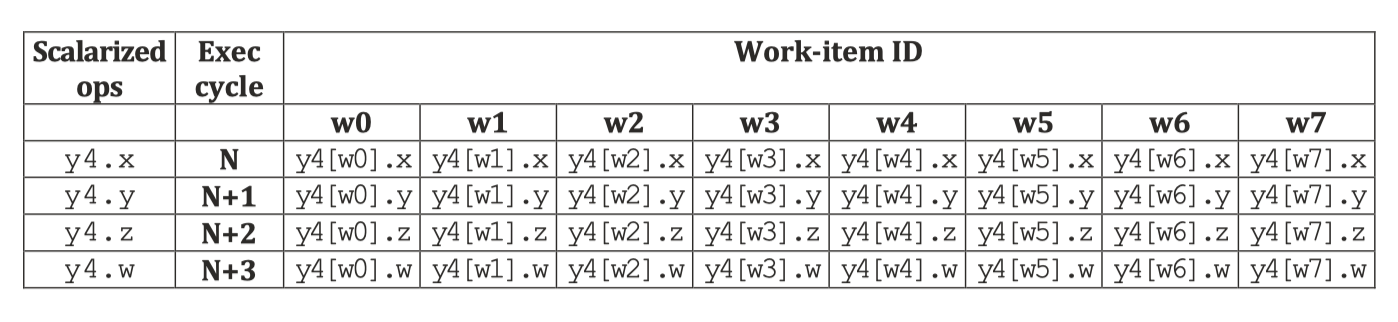
\includegraphics[width=0.9\textwidth]{figs/F11.9.png}
	\caption{\textit{任意长度输入的分层扫描。}}
\end{figure}

对于许多应用来说,扫描操作要处理的元素数量可能是数百万甚至数十亿。 
到目前为止,我们提出的内核对输入的部分执行局部块范围扫描,但我们仍然需要一种方法来合并不同部分的结果。 
为此,我们可以使用分层扫描方法,如图 11.9 所示。

对于大型数据集,我们首先将输入划分为多个部分,以便每个部分都可以放入流式多处理器的共享内存中,并由单个块进行处理。 
假设我们将图 11.3 和 11.7 中的内核之一运行在大型输入数据集上。 
在网格执行结束时,$\mathrm{Y}$ 数组将包含各个部分的扫描结果,在图 11.9 中称为扫描块。 
扫描块中的每个元素仅包含同一扫描块中所有先前元素的累加值。 
这些扫描块需要组合成最终结果; 也就是说,我们需要调用另一个内核,将前面扫描块中所有元素的总和添加到扫描块的每个元素上。

\begin{figure}[H]
	\centering
	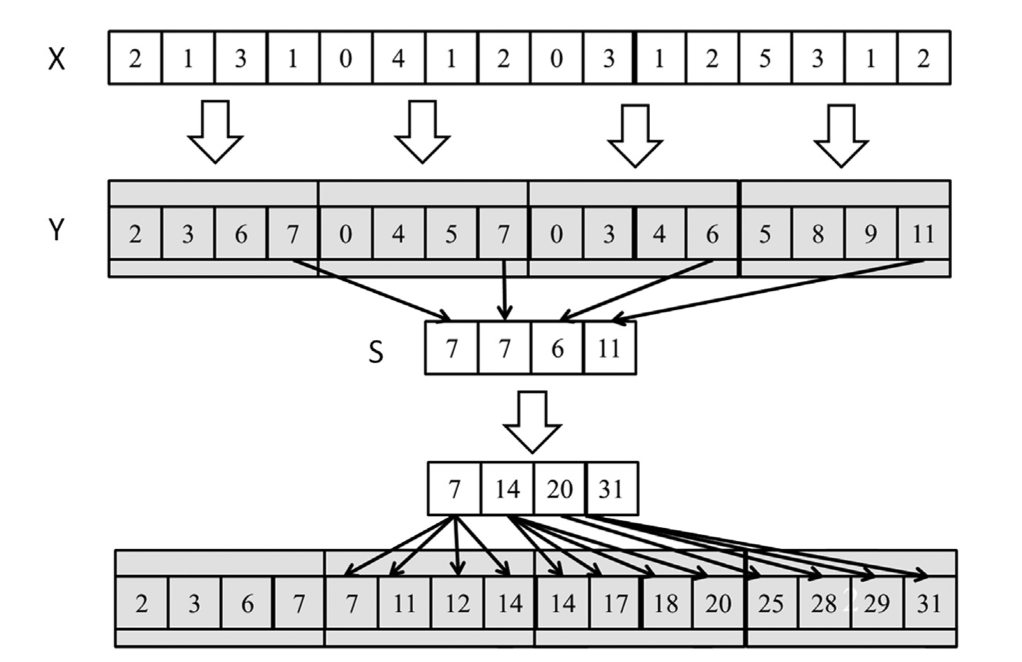
\includegraphics[width=0.9\textwidth]{figs/F11.10.png}
	\caption{\textit{分层扫描的示例。}}
\end{figure}

图 11.10 显示了图 11.9 的分层扫描方法的一个小示例。 在此示例中,有 16 个输入元素,它们被分为四个扫描块。 
我们可以使用 Kogge-Stone 内核、Brent-Kung 内核或粗化内核来处理各个扫描块。 内核将四个扫描块视为独立的输入数据集。 
扫描内核终止后,每个 Y 元素在其扫描块内包含扫描结果。 例如,扫描块 1 具有输入 $0,4,1,2$。 
扫描内核产生该部分的扫描结果,即$0,4,5,7$。 请注意,这些结果不包含扫描块 0 中任何元素的贡献。 
为了产生该扫描块的最终结果,扫描块0中的所有元素的总和,即$2+1+3+1=7$,应该被添加到扫描块1的每个结果元素。 
再举个例子,扫描块 2 中的输入是 $0,3,1,2$。 内核产生该扫描块的扫描结果,即$0,3,4,6$。 
要生成此扫描块的最终结果,应将扫描块 0 和扫描块 1 中的所有元素相加,即 $2+1+3+1+0+4+1+2=14$ 到扫描块 2 的每个结果元素。

值得注意的是,每个扫描块的最后一个输出元素给出了扫描块的所有输入元素的总和。 这些值为图 11.10 中的 7、7、6 和 11。 
这给我们带来了图 11.9 中分段扫描算法的第二步,它将每个扫描块的最后结果元素收集到一个数组中,并对这些输出元素执行扫描。 
该步骤也在图11.10中示出,其中所有扫描块的最后扫描输出元素被收集到新的阵列S中。
虽然图11.10的第二步在逻辑上与图11.8的第二步相同,但是 主要区别在于图 11.10 涉及来自不同线程块的线程。 
因此,每个部分的最后一个元素需要收集(写入)到全局内存数组中,以便它们可以跨线程块可见。

收集每个扫描块的最后结果可以通过更改扫描内核末尾的代码来完成,
以便每个块的最后一个线程使用其 blockIdx 将其结果写入 $\mathrm{S}$ 数组。 $\mathrm{x}$ 作为数组索引。 
然后对 $S$ 执行扫描操作以产生输出值 $7,14,20,31$。 
请注意,这些第二级扫描输出值中的每一个都是从每个扫描块的起始位置 $\mathrm{X}[0]$ 到结束位置的累加和。 
即$\mathrm{S}[0]=7$中的值是从X[0]到扫描块0末尾的累加和,即$X[3]$。 
$S[1]=14$中的值是从$X[0]$到扫描块1的末尾(即X[7])的累加和。 
因此,$\mathrm{S}$ 数组中的输出值给出了原始扫描问题的“战略”位置处的扫描结果。 
换句话说,在图11.10中,$\mathrm{S}[0]、\mathrm{S}[1]、\mathrm{S}[2]$
和$\mathrm{S}[3]$中的输出值分别给出原始问题在位置 X[3]、X[7]、X[11] 和 X[15] 处的最终扫描结果。 
这些结果可用于使每个扫描块中的部分结果达到其最终值。

这将我们带到图 11.10 中分段扫描算法的最后一步。 第二级扫描输出值被添加到其对应扫描块的值上。 
例如,在图11.10中,S[0]的值(值7)将被添加到$\mathrm{Y}[0],\mathrm{Y}[1],\mathrm{Y}[2], \mathrm{Y}[3]$ 线程块 1,完成这些位置的结果。 这些位置的最终结果为 $7,11,12,14$。 
这是因为 $\mathrm{S}[0]$ 包含原始输入 $\mathrm{X}[0]$ 到 $X[3]$ 的值之和。 
这些最终结果是 14、17、18 和 20。S[1] (14) 的值将添加到 Y[8]、Y[9]、Y[10]、Y[11],从而完成 这些位置的结果。 
S[2] (20) 的值将被添加到 Y[12]、Y[13]、Y[14]、Y[15]。 最后,$S[3]$的值是原始输入所有元素的总和,这也是Y[15]中的最终结果。

熟悉计算机算术算法的读者应该认识到,分段扫描算法背后的原理与现代处理器的硬件加法器中的先行进位原理非常相似。 
考虑到我们迄今为止研究的两种并行扫描算法也基于创新的硬件加法器设计,这应该不足为奇。

我们可以用三个内核来实现分段扫描。 第一个内核与三相内核基本相同。 
(我们可以同样轻松地使用 Kogge-Stone 内核或 Brent-Kung 内核。)我们需要再添加一个参数 S,
其维度为 N/SECTION\_SIZE。 
在内核的末尾,我们为块中的最后一个线程添加条件语句,
以将扫描块中最后一个 $\mathrm{XY}$ 元素的输出值写入到 S 的 blockIdx.x 位置:

\begin{figure}[H]
	\centering
	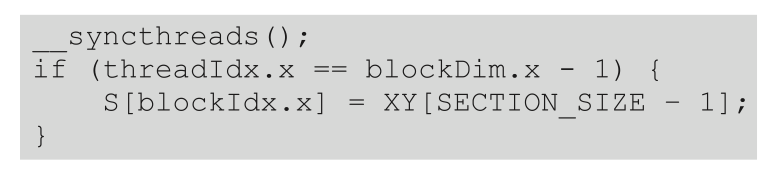
\includegraphics[width=0.9\textwidth]{figs/F11-a5.png}
\end{figure}

第二个内核只是配置有单个线程块的三个并行扫描内核之一,
它将 $\mathrm{S}$ 作为输入并写入 $\mathrm{S}$ 作为输出,而不产生任何部分和。

第三个内核将 $\mathrm{S}$ 数组和 $\mathrm{Y}$ 数组作为输入,并将其输出写回到 Y 中。
假设我们在每个块中使用 SECTION\_SIZE 线程启动内核,
则每个线程添加 $S$ 元素之一(由 blockIdx.x-1 选择)到一个 $\mathrm{Y}$ 元素:

\begin{figure}[H]
	\centering
	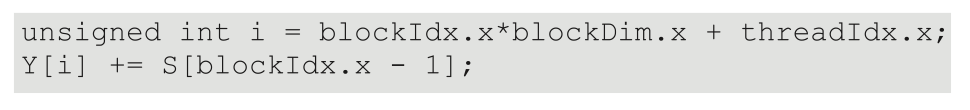
\includegraphics[width=0.9\textwidth]{figs/F11-a6.png}
\end{figure}

换句话说,块中的线程将所有先前扫描块的总和添加到其扫描块的元素中。 
我们将其作为练习,让读者完成每个内核的详细信息并完成主机代码。

\subsection{单遍扫描提高内存访问效率}
在11.6节提到的分段扫描中,部分扫描的结果(扫描块)在启动全局扫描内核之前被存储到全局内存中,
然后由第三个内核从全局内存中重新加载回来。 
执行这些额外内存存储和加载的时间不会与后续内核中的计算重叠,并且会显着影响分段扫描算法的速度。 
为了避免这种负面影响,人们提出了多种技术(Dotsenko et al., 2008; Merrill \& Garland, 2016; Yan et al., 2013)。 
本章讨论基于流的扫描算法。 我们鼓励读者阅读参考资料以了解其他技术。

在 CUDA C 编程的上下文中,基于流的扫描算法(不要与第 20 章“异构计算集群编程”中介绍的 CUDA 流混淆)
或多米诺骨牌式扫描算法是指分段扫描算法 部分和数据通过同一网格中相邻线程块之间的全局内存沿一个方向传递。 
基于流的扫描建立在一个关键观察的基础上,即全局扫描步骤(图 11.9 的中间部分)可以以多米诺骨牌方式执行,
并且并不真正需要网格范围的同步。 例如,在图11.10中,扫描块0可以将其部分和值7传递给扫描块1并完成其工作。 
扫描块1从扫描块0接收部分和值7 ,与其局部部分和值7相加得到14 ,将其部分和值14传递给扫描块2 ,
然后通过将所有部分和值加7来完成最后一步。 扫描其扫描块中的值。 对于所有线程块,此过程都会继续。

为了实现多米诺骨牌式扫描算法,可以编写一个内核来执行图 11.9 中分段扫描算法的所有三个步骤。 
线程块 $i$ 首先使用我们在 11.2 节到 11.5 节中介绍的三种并行算法之一对其扫描块执行扫描。 
然后,它等待其左邻居块 $i-1$ 传递总和值。 
一旦它收到来自块 $i-1$ 的和,它就会将该值添加到其局部和中,并将累积和值传递到其右相邻块 $i+1$。 
然后,它继续将从块 $i-1$ 接收到的总和值添加到所有部分扫描值,以生成扫描块的所有输出值。

在内核的第一阶段,所有块都可以并行执行。 它们将在数据传递阶段被序列化。 
然而,一旦每个块从其前任接收到总和值,它就可以与已从其前任接收到总和值的所有其他块并行执行其最终阶段。 
只要总和值可以快速地通过块,在第三阶段期间块之间就可以有足够的并行性。

为了使这种多米诺骨牌式扫描发挥作用,需要相邻(块)同步(Yan et al., 2013)。 
相邻同步是一种定制的同步,允许相邻线程块同步和/或交换数据。 
特别是,在扫描中,数据从扫描块$i-1$传递到扫描块$i$,就像在生产者-消费者链中一样。 
在生产者端(扫描块 $i-1$ ),在将部分和存储到内存后,将标志设置为特定值,而在消费者端(扫描块 $i$ ),
检查标志以 在加载传递的部分和之前查看它是否是该特定值。 
如前所述,加载的值进一步与局部和相加,然后传递到下一个块(扫描块 $i+1$ )。 
相邻同步可以通过原子操作来实现。 下面的代码段说明了如何使用原子操作来实现相邻同步:

\begin{figure}[H]
	\centering
	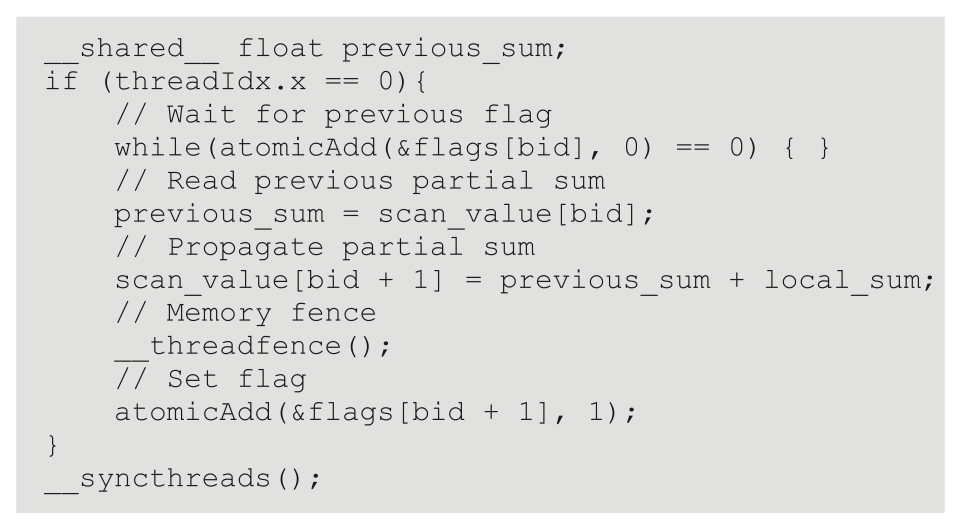
\includegraphics[width=0.9\textwidth]{figs/F11-a7.png}
\end{figure}

此代码段仅由每个块中的一个领导线程执行(例如,索引为 0 的线程)。 
其余线程将在最后一行的 \_\_syncthreads ( ) 处等待。 
在块 bid 中,领导线程会重复检查全局内存数组 flags[bid],直到其被设置。 
然后,它通过访问全局内存数组 scan\_value[bid] 加载其前一个的部分和,
并将该值存储到其局部共享内存变量 previous\_sum 中。 
它将前一个sum与其局部部分和10calsum相加,并将结果存储到全局内存数组scanvalue[bid+1]中。 
需要内存栅栏函数\_threadfence()来确保scan\_value[bid+1]值在使用atomicAdd()设置标志之前到达全局内存。

虽然对 flags 数组的原子操作和对 scan\_value 数组的访问可能会产生全局内存流量,
但这些操作大多在最新 GPU 架构的二级缓存中执行(第 9 章,并行直方图)。 
任何此类对全局存储器的存储和加载都可能与其他块的第一阶段和第三阶段计算活动重叠。 
另一方面,当执行11.5节中的三内核分段扫描算法时,全局内存中$\mathrm{S}$数组的存储和加载位于单独的内核中,
不能与阶段1或阶段1重叠。 第三阶段。

多米诺骨牌式算法有一个微妙的问题。 在 GPU 中,线程块可能并不总是根据其 blockIdx 值线性调度,
这意味着扫描块 $i$ 可能会在扫描块 $i$ +1 之后调度和执行。 
在这种情况下,调度器安排的执行顺序可能与相邻同步代码所假定的执行顺序相矛盾,从而导致性能下降甚至死锁。 
例如,调度器可以在调度扫描块$i-1$之前调度扫描块$i$到扫描块$i+N$。 如果扫描块$i$到扫描块$i+N$占用了所有流式多处理器,
则扫描块$i-1$将无法开始执行,直到其中至少一个完成执行。 然而,它们都在等待来自扫描块$i-1$的总和值。 这会导致系统死锁。

有多种技术可以解决这个问题(Gupta 等人,2012;Yan 等人,2013)。 
这里,我们只讨论一种特定的方法,即动态块索引分配,其余的留给读者参考。 
动态块索引分配将线程块索引的分配与内置 blockIdx.x 解耦。 
在单遍扫描中,每个块的 bid 变量的值不再与 blockIdx.x 的值绑定。 相反,它是通过在内核开头使用以下代码来确定的:

\begin{figure}[H]
	\centering
	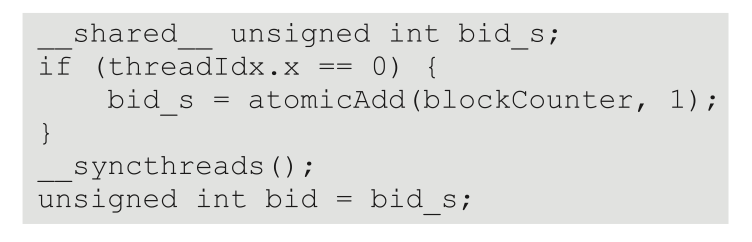
\includegraphics[width=0.9\textwidth]{figs/F11-a8.png}
\end{figure}

领导线程以原子方式递增 blockCounter 指向的全局计数器变量。 全局计数器存储被调度的下一个块的动态块索引。 
然后,领导线程将获取的动态块索引值存储到共享内存变量 bid\_s 中,
以便在 \_syncthreads() 之后该块的所有线程都可以访问它。 这保证了所有扫描块都是线性调度的并防止潜在的死锁。 
换句话说,如果一个区块获得了 $i$ 的出价值,那么就可以保证值为 $i-1$ 的区块已经被调度,因为它已经执行了原子操作。

\subsection{总结}
在本章中,我们研究了并行扫描,也称为前缀和,作为一种重要的并行计算模式。 扫描用于将资源并行分配给需求不一致的各方。 
它将看似基于数学递归的顺序计算转换为并行计算,这有助于减少许多应用程序中的顺序瓶颈。 
我们证明,简单的顺序扫描算法仅对 N 个元素的输入执行 N - 1 或 O(N) 加法。

我们首先引入了一种并行 Kogge-Stone 分段扫描算法,该算法速度快、概念简单,但工作效率不高。 
该算法执行 O (N × log2 N) 次操作,这比顺序操作要多。 
随着数据集大小的增加,并行算法与简单顺序算法保持平衡所需的执行单元数量也会增加。 
因此,Kogge-Stone 扫描算法通常用于在具有丰富执行资源的处理器中处理适度大小的扫描块。

然后,我们提出了一种概念上更复杂的并行 Brent-Kung 分段扫描算法。 
使用归约树阶段和反向树阶段,无论输入数据集有多大,该算法都仅执行 2 * N - 3 或 O(N) 加法。 
这种操作数量随输入集大小线性增长的高效算法通常也称为数据可扩展算法。 
虽然 Brent-Kung 算法比 Kogge-Stone 算法具有更好的工作效率,但需要更多步骤才能完成。 
因此,在具有足够执行资源的系统中,Kogge-Stone算法尽管工作效率较低,但仍有望获得更好的性能。

我们还应用线程粗化来减轻并行扫描的硬件利用率不足和同步开销,并提高其工作效率。 
通过让块中的每个线程在其自己的输入元素子部分上执行工作高效的顺序扫描来应用线程粗化,
然后线程协作执行工作效率较低的块范围并行扫描以生成整个块的部分。

我们提出了一种分层扫描方法来扩展并行扫描算法以处理任意大小的输入集。 
不幸的是,分段扫描算法的简单的三内核实现会产生冗余的全局内存访问,其延迟与计算不重叠。 
为此,我们还提出了一种多米诺骨牌式的分层扫描算法,以实现单通道、单内核的实现,并提高分层扫描算法的全局内存访问效率。 
然而,这种方法需要仔细设计使用原子操作、线程内存栅栏和屏障同步的相邻块同步机制。 
还必须特别注意通过使用动态块索引分配来防止死锁。

使用例如warp级洗牌操作来实现更高性能的实现还有进一步的优化机会。 
一般来说,在 GPU 上实现和优化并行扫描算法是复杂的过程,
普通用户更有可能使用 Thrust 等 GPU 并行扫描库(Bell 和 Hoberock,2012),而不是从头开始实现自己的扫描内核。 
尽管如此,并行扫描是一种重要的并行模式,它为优化并行模式的权衡提供了有趣且相关的案例研究。